% glossary.tex - thesis example with glossary
\documentclass[12pt,glossary]{dalthesis}
% to prepare draft version use option draft:
%\documentclass[12pt,draft]{dalthesis}


\usepackage{amssymb}
\usepackage{blindtext}
\usepackage{enumitem}
\usepackage[utf8]{inputenc}
\usepackage[english]{babel}
\usepackage{amsthm}
\usepackage{graphicx} %package to manage images1v
\graphicspath{ {Figures/} }
\usepackage[linesnumbered,ruled]{algorithm2e}
\usepackage{multirow}
\usepackage{setspace}
\usepackage{url}
\renewcommand{\baselinestretch}{2.0}

\newtheorem{theorem}{Theorem}[section]
\newtheorem{corollary}{Corollary}[theorem]
\newtheorem{lemma}[theorem]{Lemma}


\begin{document}

\macs  % options are \mcs, \macs, \mec, \mhi, \phd, and \bcshon
\title{COMPACT REPRESENTATIONS OF SEPARABLE GRAPHS}
\author{Xiang Zhang}
\defenceday{1}
\defencemonth{August}
\defenceyear{2017}
\convocation{September}{2017}

% Use multiple \supervisor commands for co-supervisors.
% Use one \reader command for each reader.

\supervisor{Dr. Meng He}
\reader{D. Odaprof}
\reader{A. External}



\frontmatter





\begin{abstract}
Much work has been conducted to represent graphs succinctly, which means encoding the graphs in a compact representation whose space cost is close to the information-theoretic lower bound, and this representation still supports efficient query operations. A previous approach by Blandford $et \ al.$~\cite{compact-representation} based on adjacency table representation makes use of small separators of a separable graph to represent the graph compactly. This representation uses $O(n)$ bits if the input graph has a vertex separator of size $O(n^{c})$, where $n$ is the number of vertexes in this graph and $c$ is a constant in (0,1), meanwhile using constant time to support degree or adjacency queries as well as constant time per neighbour for neighbour listing operations.


We implemented a practical variant of this data structure based on edge separators. The data structure was built by recursively partitioning a graph. We stored a compressed adjacency list for each vertex, and then concatenated the adjacency lists in the order of the number assigned to each vertex based on the recursive partition to form an adjacency table. Then we implemented several indexing structures to support general queries on graphs. We conducted some experiments to measure the performance of this representation as well as the performance of standard array-based adjacency list representation. The experiment shows our implementation reduces space usage by almost an order of magnitude, while supporting Bread-first-search in acceptable running time when compared to the array-based representation.
\end{abstract}

\printglossary

\begin{acknowledgements}
My supervisor, Dr. Meng He, deserves the most praise for his invaluable guidance, friendship and suggestions. I would also like to thank all of the friends and acquaintances I have made at Dalhousie University. They have made this journey something to remember. Without everyone’s support and guidance this project would have not been a success.
I would like to thank Dalhousie University to provide such a great environment
to do research and allowing me to finish my work.
I am proudly grateful to my supportive and loving family for their whole-hearted
support of my graduate studies.
\end{acknowledgements}

\mainmatter

\chapter{Introduction}

Nowadays, many applications use graphs to show the relationship and represent connectivity between multiple objects. The usage of such graphs is so popular in representing various data types including link structures of the web, 3d mesh models, geographic maps, and surface meshes in computer graphics. As the graphs inevitably grow very huge, the space issue becomes ever more important. Hence, the problem of designing space-efficient data structures to represent graphs while supporting efficient queries operations has drawn a great deal of attention. 

\bigskip
Much works has been conducted to represent graphs succinctly, which means encoding the graphs in a compact representation whose space cost is close to the information-theoretic lower bound, and this representation still supports efficient query operations. The problem of succinctly representation of a graph can be formalized as: Given a graph $G = (V, E)$ of type $\chi$, where $n$ and $m$ are numbers of vertexes and edges, respectively, represent $G$ using $\lg | \chi | + o(\lg | \chi | )$ bits of space, where $|\chi|$ is the number of different graphs of type $|\chi|$ , and support a set of query operations on the graph in constant time (assuming we can access $\Theta(\lg n)$ consecutive bits in one operation). Because the space bound may not be satisfied, therefore, the trade-off between space cost and query time can be further investigated.  

\bigskip


A considerable strategy to save the space when representing graphs is taking advantage of structural properties of graphs. In practice, the most common structural property of graphs is that they have small separators. A graph has separators if it can be partitioned into two subgraphs of approximately equal size by removing a few vertexes. For example, planar graphs, have $O(n^{1/2})$ sized separators, and even graphs that are not strictly planar because of crossings, such power networks, have small separators too. More generally, nearly all graphs that represent connections relationship in low dimensional spaces have small separators. We say a graph is separable if it is taken from a class of graphs that satisfies an $n^{c}$-separator theorem~\cite{separator-theorem} for some constant c $<$ 1.

\bigskip


In this project, we are interested in improving a compact representation mechanism for separable graphs presented by Blandford $et \ al.$~\cite{compact-representation}, in which the authors proposed an approach to represent separable graphs compactly based on an adjacency list representation. Their representation used $O(n)$ bits if the input graph has a vertex separator of size $O(n^{c})$, where $n$ is the number of vertexes in this graph and $c$ is a constant in (0,1), meanwhile using constant time to support degree or adjacency queries, as well as constant time per neighbour for neighbour listing queries (They took advantage of $O(\lg n)$-bit parallelism computation to access $\Theta(\lg n)$ consecutive bits in one operation). For graphs with small separators, their representation achieved good compression ratios, and even for graphs that were not strictly separable, their representation still worked well because the separable components in those graphs can be compressed. In their paper, they provided a detailed description for compressing the graph by building two structures: the adjacency table and the root-find structure, which used vertex separators to encode the graph into a shadow adjacency table, and to support query operations in constant time. But in their experimental studies, they implemented the data structure using edge separators instead of vertex separators, which means the shadow label and root-find structure were not needed. This simplification is needed because these two data structures are not practical. In this project, we implemented the data structure by using edge separators, and conducted experiments on it.

\bigskip
\bigskip

We firstly followed their idea to implement the data structure by using edge separators. The data structure was built by recursively partitioning a graph into two subgraphs until each subgraph has only one vertex. During the partition process, an edge separator tree was built. Then we made use of the edge separator tree to renumber the vertexes. We stored an adjacency list for each vertex, and then concatenated the adjacency lists in the order of the number assigned to each vertex in the renumbering process to form an adjacency table. Each pair of vertexes in the adjacency was stored by encoding the difference $d$ between the two vertexes, and all the differences were stored contiguously as a sequence of bits in memory. We proved, using this approach, $O(n)$ bits were sufficient to encode the separable graph. 

\bigskip
\bigskip

Next, we implemented several indexing structures to support degree and adjacency queries in constant time, and neighbour listing in constant time per Neighbour. These indexing structures include all the structures used in their experiment, as well as two indexing structures based on succinct bit vectors. In their paper, they encoded the degree of each vertex at the start of each adjacency list. However, the space of degree could be saved in some cases, which yielded a trade-off between the time to support degree queries and the space to encode the graph in our studies.

\bigskip
\bigskip

Finally, We compared the performance of various indexing structures by conducting a Bread-first search in the graphs. We also compared our space and time cost to those of an array-based adjacency list representation. The result showed that our implementation save a magnitude of space when compared to standard array-based adjacency list, while supporting efficient queries.   

\section{Related Work}

There has been considerable work dedicate to compressing graphs such as planar graphs, k-page graphs and separable graphs. The first attempt of succinct representation of graphs was conducted by Jacobson~\cite{Jacobson}, who first showed how to represent a planar graph on $n$ vertexes using $O(n)$ bits while supporting adjacency queries in $O(\log n)$ time. His approach decomposed a planar graph into at most four one-page graphs which are represented as a sequence of balanced parentheses. His representation extended naturally to a $k$-page graph, where k$\geq$1. A k-page graph is a graph which consists of k outerplanar graphs sharing the same spine. k-page graphs can be considered as undirected graphs or as directed graphs where an edge always goes from a smaller-numbered to a larger-numbered vertex, and a planar graph has at most 4 pages~\cite{k-page-def}. 

\bigskip
\bigskip

Munro and Raman~\cite{Munro} improved the time for adjacency queries to O(1) time while using $8n+2m$ bits to represent a planar graph, where $n$ and $m$ are numbers of vertexes and edges, respectively. Their work greatly reduced the number of bits regarding Jacobson's representation. Geary $et$ $al.$~\cite{Geary} gave a conceptually simpler representation compared to Jacobson's data structure which used $2n+o(n)$ bits. The space constants on the high order term had been improved by Chuang $et$ $al.$~\cite{Chuang}, and further by Chiang $et$ $al.$~\cite{Chiang}, which used $\frac{3}{5} m + (5+ \epsilon )n + o(n)$ bits and  $2m+2n+O(m+n)$ bits, respectively. The former proposed another encoding mechanism based on $canonical \ orderings$ of a planar graph, and then used a $multiple \ parentheses \ sequences$ to represent the graph, while the latter generalized the notion of canonical orderings to orderly spanning trees and improved constant factors in terms of numbers of vertexes and edges. 

\bigskip
\bigskip

A succinct representation of a k-page graph for large k that supports various navigational operations more efficiently, was proposed by Barbay $et$ $al.$~\cite{Barbay}, whose representation used $n+2m\lg n + m \cdot o(\lg k) + o(m)$ bits to support adjacency queries in $O(\lg k \lg \lg k)$ time, degree queries in constant time and neighbourhood in $O(d(x) \lg \lg k)$ time, where $d(x)$ is the degree of vertex $x$, or used $n+(2+\epsilon)m\lg k + m \cdot o(\lg k) + O(m)$ bits to support adjacency, degree and neighbourhood queries in $O(\lg k)$, $O(1)$ and $O(d(x))$ time, respectively, where $\epsilon$ is any constant that satisfies $0< \epsilon <1$.   

\bigskip

\begin{table}[ht]
\small
\centering
\caption{A summary of performance of various of succinct planar graph representations. Notation: "Pla*" indicates the planar graphs, "k-p*" indicates k-page graphs, "Tri*" indicates planar triangulations, "Sep*" indicates separable graphs, $n$ and $m$ denote the numbers of vertexes and edges in Graph $G$, respectively, $i$ is the number of isolated vertexes in $G$, $\epsilon$ is an arbitrary positive constant, $\tau$ = min\{ $\lg k / \lg \lg m, \lg \lg k$\} }. 
\label{my-label}
\begin{tabular}{|c|c|c|c|c|c|}
\hline
Type                       & Ref. & Space & Adjacency & Neighborhood & Degree \\ \hline
\multirow{4}{*}{Pla*}    &  ~\cite{Jacobson}    & $O(n)$ &   $O(\lg n)$   &       $O(deg(x) \lg n)$       &    $0(\lg n)$    \\ \cline{2-6} 
                           &   ~\cite{Chuang} &  $\frac{3}{5} m + (5+ \epsilon )n + o(n) $  & $O(1)$  & $O(deg(x))$ &   $O(1)$     \\ \cline{2-6} 
                           & ~\cite{Chiang} & $2m+2n+0(m+n)$& $O(1)$  &  $O(deg(x))$  &  $O(1)$     \\ \cline{2-6} 
                           & ~\cite{Munro} & $2m+8n+o(n)$&  $O(1)$  &  $O(deg(x))$  &   $O(1)$  \\ \hline
\multirow{5}{*}{k-p*}    &  ~\cite{Jacobson} &  $O(kn)$  & $O(\lg n + k)$  &  $O(geg(x)\lg n$  &  $O(\lg n)$ \\ \cline{2-6} 
                           &   ~\cite{Gavoille}   & $(2(m+i)+o(m+i))\lg k$ & $O(\tau \lg k)$  &  $O(deg(x) \tau)$ & O(1) \\ \cline{2-6} 
                           &  ~\cite{Barbay} & $2m \lg k+n+o(m \lg k)$  & $O(\lg k \lg \lg k)$  & $O(deg(x) \lg \lg k)$ &   $O(1)$  \\ \cline{2-6} 
                           &   ~\cite{Barbay}   & $(2+\epsilon )m\lg k+n+o(m\lg k)$ & $O(\lg k)$ & $O(deg(x))$& $O(1)$        \\ \cline{2-6} 
                           &~\cite{Munro} & $2m+2kn+o(kn)$ & $O(k)$  & $O(deg(x)+k)$ &  $O(1)$  \\ \hline
\multirow{1}{*}{Tri*} &  ~\cite{Chuang}    & $2m+n+o(n)$  & $O(1)$      & $O(deg(x))$    & $O(1)$   \\ \hline
                           
\multirow{2}{*}{Sep*} &  ~\cite{compact-representation}    & $O(n$)  & $O(1)$      & $O(deg(x))$    & $O(1)$   \\ \cline{2-6} 
                           &  ~\cite{succinct-representation}    &  $o(n)+ \lg |\chi|$     & $O(1)$      & $O(deg(x))$    & $O(1)$   \\ \hline
\end{tabular}
\end{table}






\bigskip

Blandford $et$ $al.$~\cite{compact-representation} showed how to use $O(n)$ bits to represent graphs that satisfies an $n^{c}$-separator theorem, while supporting degree and adjacency queries in $O(1)$ time, and neighbourhood queries in constant time per neighbour. Subsequently, Blelloch $et$ $al.$~\cite{succinct-representation} proposed a succinct representation of unlabelled separable graphs, which used $lg| \chi |+ o(n)$ bits to represent a graph of type $\chi$, while holding the same time bounds as the performance of Blandford's representation. A summary of the performance of various of succinct planar graph representations is shown in Table 1.1.
        

\section{Outline}
The rest of this report is organized as follows. Chapter 2 provides some background information for this project. Chapter 3 describes the compressed graph representation by Blandford $et \ al.$~\cite{compact-representation}, including the construction and usage of the edge separator tree as well as those of several indexing structures. Chapter 4 describes the experimental setup and examines the performance of our implementation. Chapter 5 shows the conclusion as well as the future work of our project.


\chapter{Preliminaries}

This chapter introduces some concepts in information theory and some data structures which are used in our work, including the concept of the graph separator, basic query types in graphs, bit vectors used in our implementation and the adjacency tables which can represent a graph.

\section{Graph Separators}
A family of graphs $G$ satisfies the $f(.)$-separator theorem ~\cite{separator-theorem} if there are constants $\alpha$ $<$ 1 and $\beta$ $>$ 0 such that each member graph in $G$ with $n$ vertexes has a separator set $S$ of at most $\beta f(n)$ vertexes whose removal partitions the graph into two parts A and B, with at most $\alpha n$ vertexes in each.

\bigskip
\bigskip

In this project we focus on the graphs that satisfy the $n^{c}$-separator theorem for some constant $c < 1$, which means the graphs have a small separator of size $O(n^{c})$, and we will say a graph is separable if it is in a class of graph which satisfies the $n^{c}$-separator theorem. One class of graphs that satisfies this condition the planar graphs, which satisfies the theorem with $c = \frac{1}{2}$ . Another example can be well-shaped meshes in $\mathbb{R}^{d}$ , with separators of size $O(n^{1-1/d})$~\cite{ separators-sphere-packing}.  Lipton $et \ al$.~\cite{Nested-Dissection} proved that all classes of graph which satisfy the $n/(\log n )^{1+\epsilon}$-separator theorem have bounded density, a graph on $n$ vertexes has bounded density if it has $O(n)$ edges. So we can assert that separable graphs have bounded density.

\bigskip
\bigskip

By making use of the definitions above, we say that a class of graphs G satisfies the $f(n)$-edge separator theorem if there are constant variables $\alpha$ $<$ 1 and $\beta$ $>$ 0 such that each member graph in $G$ with $n$ vertexes has an edge separator with at most $\beta f(n)$ edges whose removal partitions the graph into two subgraphs with at most $\alpha n$ vertexes in each. The edge separator is not as common as the vertex separator, because a graph with an edge separator of size $s$ also has a vertex separator of size s at most, but no similar bound holds when it is conversed~\cite{compact-representation}.

\bigskip
\bigskip

In this project, we only considered the undirected connected graph, which meant all vertexes in the graph have nonzero degrees, and we assumed each step of partitioning always returns a edge separator set of size $O(n^{c})$.

\bigskip
\bigskip

\section{Queries in Graphs}
Our data structure supports three kinds of queries on separable graphs: adjacency queries, degree queries and neighbour listing. The adjacency query checks whether there is an edge between two vertices, the neighbour listing returns the neighbours of a given vertex, and the degree query reports the number of edges connected to a given vertex.

\bigskip
\bigskip

\section{Bit Vectors}
The compact representation stores a separable graph as a difference-encoded bit sequence in memory. To support the three kinds queries (adjacency queries, degree queries and neighbour listing) in constant time, knowing both the number of encoded adjacency lists in the sequence up to an index position, and the starting position of a particular adjacency list is necessary. More formally, the compact representation requires data structures that support rank and select operations in constant time: Given a bit vector $B[0...n)$ represents a subset $S$ of a universe $U = [0...n)$ = $\{0,1,...,n-1 \}$, where $B[i] = 1 \ iff \ i \in S$, we define the following two operations, 

\begin{itemize}[noitemsep]
\item $rank_{q}(x)$ = $\{k \in [0...x] : B|k| = q \}$
\item $select_{q}(x)$ = $ min \{ k \in [0...n) : rank_{q}(k) = x \} $ 
\end{itemize}


In this project, we used two different succinct representations of bit vectors: RRR~\cite{RRR} and SD vector~\cite{SD-vector} in order to build two indexing structures that supports queries in a separable graph. Both structures match the information-theoretic lower bound on representing a bit vector, and still support efficient rank and select query operations. More detail about these two structures will be given in section 3.3, where we use them to build indexing structures.

\bigskip
\bigskip
\section{Adjacency Tables}
An adjacency list representation for a graph associates each vertex in the graph with the collection of its neighbouring vertices. when used as a data structure, the main alternative to the adjacency list is the adjacency matrix. For a sparse graph (most pairs of vertices are not connected by edges) and especially a graph with $bounded \ density$, an adjacency list representation is significantly more space-efficient than an adjacency matrix representation: the space cost of the adjacency list representation depends on the number of edges and vertices in the graph, while the adjacency matrix representation is stored as the square of the number of vertices. Generally, if we encode the neighbours of each vertex in an array of 32-bit integers, an adjacency list representation for an undirected graph requires 8$|E|$ bytes (2*32*$|E|$ bits) of space, where $|E|$ is the number of edges in the graph. However, it is not space-efficient enough yet. In chapter 3, we show how Blandford $et \ al$~\cite{compact-representation} further improved the space efficiency.



\chapter{Compressed Representation of Separable Graphs}

Blandford $et \ al.$~\cite{compact-representation} chose to describe their theoretical solution based on vertex separators first. Then, as this solution is not practical, they gave some brief guidelines on how to simplify it for graphs with small edge separators before implementing it for an experimental study. Here we directly introduce the practical solution based on edge separators in details, without introducing the theoretical solution based on vertex separators first. Thus, anyone interested in using these solutions in practice can read this chapter to learn the details, without having to work out the details by themselves. In addition, for a postprocessing step called child flipping which is for the construction of this data structure, Blandford $et \ al.$~\cite{compact-representation} only described the corresponding heuristics, without saying how to perform this step efficiently. Thus, we will describe our implementation of this step in details in this chapter. The content of this chapter includes the process of generating a separator tree from the input graph to renumber the vertexes, a postprocessing stage algorithm to further reduce the space needed to encode the adjacency table, as well as several indexing structures to support efficient graph queries meanwhile using less space.    


\section{Building an Edge Separator Tree}

\textbf{Edge Separators}. To compactly represent a graph, the first thing we need to do is building an edge separator tree from the input graph. The tree-building process is based on recursively partitioning the graph into two subgraphs using the edge separator. One example that illustrates the function of edge separators is shown in Figure 2.1: Assuming we have an 8-vertex graph $G_{1}$ with 9 edges, by removing the two edges $(v_{1}, v_{8})$ and $(v_{1}, v_{5})$, we can partition $G_{1}$ into two subgraphs with 4 vertexes in each. Hence the edge separator in this partitioning step is $\{(v_{1}, v_{8}),(v_{1}, v_{5}) \}$.

\bigskip

\begin{figure}[ht]
\centering
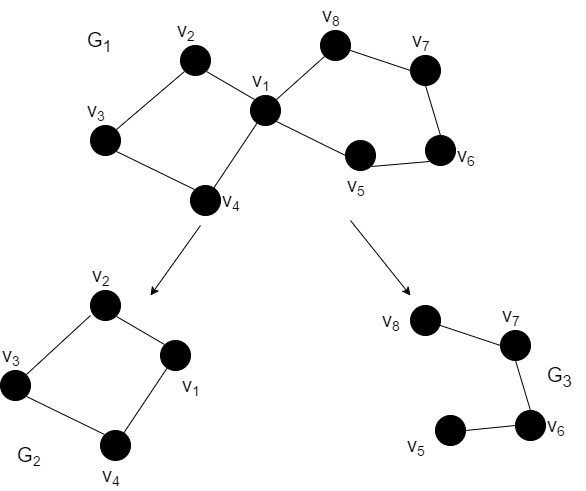
\includegraphics[width=0.7\textwidth]{partition}
\caption{An example of a partition process of using edge separators}
\end{figure}

\bigskip

We can see that each time we partition a graph, it splits its vertex set and part of its edge set, and removes some edges. if we perform this partitioning recursively until each subgraph has only one vertex, then we have an edge separator tree from the graph. One edge separator tree for the graph $G_{1}$ in Figure 2.1 is shown in Figure 2.2. Each vertex in a graph will appear once in a leaf of the edge separator tree build from that graph. Each internal node is the set of edges used as the edge separator to partition the corresponding subgraph.

\begin{figure}[ht]
\centering
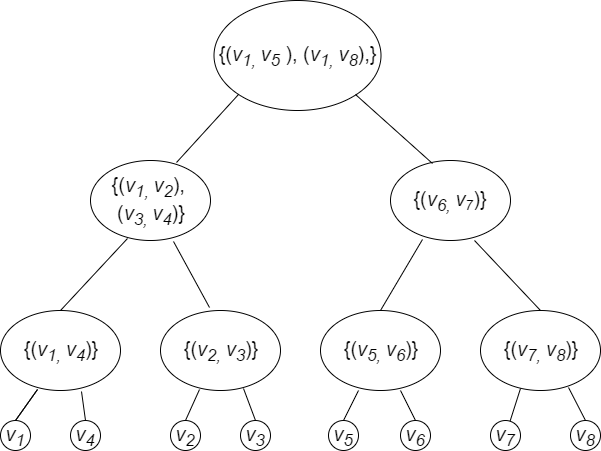
\includegraphics[width=0.8\textwidth]{separatorTree}
\caption{An example of edge separator tree}
\end{figure}

\bigskip
\bigskip
Note that we arbitrarily decided which side of the partition will be the left child or the right child at this stage. We will take advantages of this "freedom" to further reduce the space needed to encode the graph in section 3.2. The tree is also not perfectly balanced in some cases (e.g. it is possible that one child is a leaf and the other is an internal node). We then make use of the edge separator tree to renumber the vertexes of the input graph as follows: perform an in-order traversal of this tree. Each time we encounter a leaf node, we retrieve the single vertex of the subgraph that corresponds to this leaf.We then list the vertexes of the graphs in the order in which they are retrieved during this traversal, renumber the first vertex in this ordering as vertex 1, and renumber other vertexes incrementally. For example, in Figure 2.2 the vertexes $v_{1}$, $v_{4}$, $v_{2}$, $v_{3}$, $v_{5}$, $v_{6}$, $v_{7}$, $v_{8}$ are renumbered as $v_{1}$, $v_{2}$, $v_{3}$, $v_{4}$, $v_{5}$, $v_{6}$, $v_{7}$, $v_{8}$, respectively.

\bigskip
\bigskip

\textbf{METIS Partition Library}. To recursively partition a given graph, we used METIS's API~\cite{metis-lib} in our project. METIS is an open source library developed by Karypis lab at the University of Minnesota. It provides a of serial programs for partitioning graphs such as finite element meshes. The algorithms implemented in METIS are based on the multilevel recursive-bisection, multilevel k-way, and multi-constraint partitioning schemes [2]. The METIS partitioning API returns one integer list with vertex index as the key, and a flag 0 or 1 to indicate which of the the two subgraphs that the original graph is partitioned into contains this vertex. The returned value of METIS API does not provide information about edges, and the API takes two integer arrays (the adjacency list of current graph and the indices of vertexes in the adjacency list) as input parameters, and hence, before each of the METIS API, we need to generate an adjacency list and a vertex index list for the current graph to be partitioned. In order to determine the set of edges that forms the edge separators, we need both the adjacency list and the returned values after calling the API.

\bigskip
\bigskip

The algorithm used to build the separator tree is given in Algorithm 1. Here we use $(V,E)$
to represent a graph for simplicity, but in fact, the METIS API takes a formalized adjacency list and the a vertex index list as input parameters. Therefore, each time we call the METIS API, the current vertex set needs to be renumbered temporally by contiguous ascending numbers, and the adjacency list needs to be initialized accordingly. The METIS API also does partition a graph with fewer than 3 vertexes, and therefore, we write additional code for such graphs.

\bigskip

\begin{algorithm}
    \underline{buildTree} $(V,E)$\;
    \eIf{$|V|=1$}
      {
        return $V$\;
      }
      {
      	$(V_{a},V_{b})$ $\leftarrow$ \textbf{METIS$\_$API} $(V,E)$  \;
		$E_{sep}$ $\leftarrow$ \textbf{findEdgeSeparator} $(V,E,V_{a},V_{b})$ \;
		$E'$ = $E \  - \ E_{sep}$   \;
      	$E_{a}$ $\leftarrow$ $\{ (u,v) \in E' \ | \  u\in V_{a} \vee v \in V_{b} \}$ \;
		$E_{b}$ = $E'$ - $E_{a}$ \;
		$T_{a}$ $\leftarrow$ \textbf{buildTree} $(V_{a},E_{a})$ \;
		$T_{b}$ $\leftarrow$ \textbf{buildTree} $(V_{b},E_{b})$ \;  
        return \textbf{separatorTree} $(T_{a}, E_{sep}, T_{b})$ \; 
      }
    \caption{Building the edge separator tree. The variables $V_{a},\ V_{b}$ represent the vertex set of two subgraphs, respectively. The $findEdgeSeparator$ function exams the original graph and the partitioning result to determine the edge separator. The $separatorTree$ function builds the tree-like structure based on the partitioning result.}
\end{algorithm}
\bigskip

\textbf{Building the Adjacency Table}. After getting the edge separator tree, we needed to renumber the vertexes based on an in-order traversal along the tree. A mapping table is also generated after completing the traversal, which will be used to build an adjacency list for each renumbered vertex using the new vertex labels. For each vertex, we stored an adjacency list which contains its all neighbouring vertexes. If a vertex with label $v$ has neighbours $v_{1}, v_{2}, v_{3}, ...,v_{n}$ in ascending sorted order, then we encoded the difference between each adjacent pair in the adjacency list as $|v_{1}-v|, \ |v_{2}-v_{1}|,\  |v_{3}-v_{2}|,\ ...,\ |v_{n}-v_{n-1}|$ contiguously, which forms a sequence of bits stored in memory. We used the Elias gamma code~\cite{Gamma} to encode the differences, which uses $2\lfloor \log n \rfloor + 1$ bits to encode a difference. The difference $v_{1} - v$ may be negative in some cases, so we here stored a one-bit flag to indicate whether the value is positive. To facilitate the degree queries, the degree of each vertex needs to be encoded at the starting position of the corresponding adjacency. By concatenating all the adjacency lists in the order of the vertex labels, we formed an adjacency table. To access the adjacency list of a vertex, knowing the starting position of the adjacency is necessary. The easiest and fastest approach is to store an array of offset pointers of size $O(\log (n))$ for each. But if we do so, we would use $O(n\log (n))$ bits of space, which exceeds our space bound. Alternatively, we implemented other two indexing structures proposed by Blandford $et \ al$~\cite{compact-representation}, as well as two indexing structures based on succinct representation of bit vectors, which brings less space cost down to $O(n)$ bits.

\bigskip
\begin{lemma}
The adjacency table constructed in this section can support degree queries in $O(1)$ time, and neighbour
listing in $O(d)$ time, where $d$ is the degree of the vertex.
\end{lemma}
\bigskip 
\begin{proof}
To access an adjacency list of a particular vertex, we use our indexing structures to locate its starting position in constant time. Each adjacency list consists of an encoded degree number and a sequence of encoded differences, which use $O(\log n)$ bits and $O(d\log n)$ bits respectively, where d is the degree of the vertex. By taking advantages of the $O(\log n)$-bits parallelism computation, we can decode any $O(\log n)$-bits value in constant time using a lookup table. Hence we can decode the degree at the starting of each adjacency list in constant time. For neighbour listing, we decode each difference pair in constant time. So it takes constant time to answer degree queries, and $O(d)$ time to answer neighbourhood queries.
\end{proof}

\bigskip
\begin{lemma}
Any n-vertex member in a class of graphs which satisfies an $n^{c}-edge$ separator
theorem can be encoded in $O(n)$ bits using the approach described in this section.
\end{lemma}

\bigskip
\begin{proof}
For each edge $(u, v)$ in an edge separator in a graph with s vertexes, the difference
between vertex u and vertex v is $O(s)$. We use gamma codes to encode the difference which would use $O(\log (s))$ bits, so that edge will contribute $O(\log (s))$ bits to the adjacency lists of both vertex u and vertex v. Hence, we charge $O(\log (s))$ to every edge in a separator of a graph with s vertices. Recall that by using the $n^{c}- edge$ separator theorem, each member with $n$ vertexes in the class of the graph has a $\beta n^{c}$ edge separator whose removal partitions the member into two parts with at most $\beta n$ vertexes in each. Let us define $S(n)$ to be an upper bound of required bits to encode a graph with n vertexes, and let $\alpha < a < 1 - \alpha $, then $S(n)$ satisfies the recurrence:
\[ S(n) \leq S(an) + S(n-an) + O(n^{c} \log n) \]
This recurrence can be solved to $S(n) = O(n)$, and the bits to encode the degree of all the vertexes is bounded by $O(n)$, because there are $O(n)$ edges in total. Therefore, the total space is $O(n)$ bits.
\end{proof}

\bigskip
\bigskip

\section{Post Processing}

\textbf{Child-flipping Algorithm}. When encoding the graph, we contiguously encode the difference between each adjacent pair in the adjacency list by using gamma codes. The gamma codes use $2\lfloor \log d \rfloor + 1$ bits to encode a difference $d$. If we can make each difference "smaller", in other words, if we can make the labels of vertexes in an adjacency list closer to each other, and then we can reduce the space to encode the adjacency list. We arbitrarily decide the side of partitioning during the construction of the separator tree (in our project, we decided the side of partitioning according to the output value of METIS API: if a 0 bit is assigned to a vertex, then it is placed in the subgraph corresponding to the left child, otherwise, it is in the subgraph for the right child), so there is a degree of freedom in the way to build the tree. To take advantage of this freedom, we can apply a heuristic optimization method called "child-flipping"~\cite{compact-representation} to our edge separator tree.

\bigskip
\bigskip

The child-flipping algorithm works as follows: when making traversal along a separator tree, it tracks the nodes containing vertex labels which appear before and after the vertex labels in the current node. For simplicity, we say that a graph vertex $v$ is in a node $x$ of the separator tree if $v$ is contained in the subgraph corresponding to $x$. Let us define $N_{L}$ to be the left children of current node's left ancestors and $N_{R}$ to be the right children of the current node's right ancestors, $N_{1}$ and $N_{2}$ represent the current node's left child and right child, respectively, and $E_{AB}$ indicates the number of edges between the vertexes in node A and node B. For each node, the vertexes in $N_{1}$ of the current node will have labels less than the vertexes in $N_{2}$, and there is no intersection between the vertexes in $N_{L}$ and $N_{R}$ of the node. The child-flipping exams $E_{N_{L}N_{1}}$, $E_{N_{2}N_{R}}$, $E_{N_{L}N_{2}}$ and $E_{N_{1}N_{R}}$ of each node to ensure that $E_{N_{L}N_{2}} + E_{N_{1}N_{R}} \leq E_{N_{L}N_{1}} + E_{N_{2}N_{R}}$. If not, the child-flipping algorithm swaps the two children of current node. The initiation of making this swap is: after renumbering the vertexes based on an in-order traversal, if $E_{N_{L}N_{1}} + E_{N_{2}N_{R}} < E_{N_{L}N_{2}} + E_{N_{1}N_{R}}$, then the space to encode the edges $E_{N_{L}N_{2}}$ and $E_{N_{1}N_{R}}$ is greater than that to encode $E_{N_{L}N_{2}}$ and $E_{N_{1}N_{R}}$, because the difference between a vertex in $N_{2}$ and a vertex in $N_{L}$ is obviously greater than the difference between a vertex in $N_{1}$ and a vertex in $N_{L}$, similar fact works on the difference between the vertexes in $N_{R}$ and vertexes in $N_{1}$ and the difference between the vertexes in $N_{R}$ and vertexes in $N_{2}$.

\bigskip
\bigskip

\textbf{Speed Up the Child-flipping Algorithm}. This heuristic algorithm can be applied to any edge separator tree as a postprocessing step. However, this process is quite time-consuming, and the time cost of applying both METIS and child-flipping in Blandford $et \ al.$~\cite{compact-representation}'s experiment demonstrates this. To get the four numbers of edges ($E_{N_{L}N_{1}}$, $E_{N_{2}N_{R}}$, $E_{N_{L}N_{2}}$ and $E_{N_{1}N_{R}}$), we need to have the four vertex sets: $N_{L}$, $N_{R}$, $N_{1}$ and $N_{2}$ for each tree node. $N_{L}$ and $N_{R}$ of each node in separator tree can be computed, but $N_{1}$ and $N_{2}$ need to be calculate locally when reaching the node. In our project, we made some efforts to reduce the time to conduct this child-flipping process: Let's assume we have a node $a$ in a separator tree with left child as $b$ and right child as $c$. If we knew the $N_{1}$ and $N_{2}$ sets of $a$ (denote as $N_{1a}$ and $N_{2a}$, and here we use $N_{La}$ and $N_{Ra}$ to represent $N_{L}$ and $N_{R}$ sets of $a$), then

\begin{itemize}[noitemsep]
\item for node b : $ N_{1b} = N_{1a}, N_{2b} = N_{2a} \cup N_{Ra}$
\item for node c : $ N_{1c} = N_{1a} \cup N_{La}, N_{2c} = N_{2a}$ 
\end{itemize}

Having this general case,  we can generate the $N_{1}$ and $N_{2}$ sets for each node during the child-flipping traversal via DFS. The $N_{L}$ and $N_{R}$ sets of each node in separator tree can be computed via a post-order traversal along the edge separator tree; the $N_{L}$ or $N_{R}$ set of a tree node is formed by merging the $N_{L}$ or $N_{R}$ set of its left or right child and is stored as a sorted array. Then we can get the $N_{1}$ and $N_{2}$ sets of a node by merging the $N_{L}$ or $N_{R}$ set of its parent node into $N_{1}$ or $N_{2}$ set of its parent node. Note that here we maintained the $N_{1}$ or $N_{2}$ set as a set of sorted array instead of just one long sorted array, and each sorted array is a $N_{L}$ or $N_{R}$ set of an ancestor of the current node. When counting the four edge numbers ($E_{N_{L}N_{1}}$, $E_{N_{2}N_{R}}$, $E_{N_{L}N_{2}}$ and $E_{N_{1}N_{R}}$), we check an existing of an edge by performing binary search for one vertex in $N_{1}$ or $N_{2}$ set on the $N_{1}$ or $N_{2}$ set of the current node. The height of tree is $\lg n$, which means there are $\lg n$ sorted lists in a $N_{1}$ or $N_{2}$ set, and the time cost of a binary search on an $n-element$ sorted array is $O(\lg n)$, and hence it takes $O(\lg ^{2} n)$ time for each edge finding. All of above approaches improve the speed of child-flipping processing significantly.

\section{Indexing Structures}

We have already described how to encode a graph with a good edge separator into an adjacency table bounded by $O(n)$ bits, but to access the particular adjacency list for a particular vertex, we need to know the exact starting position in the bit sequence. Hence our representation requires a data structure that supports efficient select operations on the bit sequence. Ideally, the space cost of the data structure should not exceed our space bound which is $O(n)$. Blandford $et \ al.$ had proposed three kinds of indexing structure: $direct$, $semi-direct$, and $indirect$~\cite{compact-representation} to support efficient select queries. In addition to these three structures, we also implement two other indexing structures based on RRR and SD Vector, respectively, and we will henceforth call these two RRR-based and SDV-based indexing structures. We will introduce all the five indexing structures in this section.

\bigskip
\bigskip

\textbf{Direct indexing structure}. The easiest way to access the starting position of 
any adjacency list is to store an offset pointer for each vertex. Because our representation uses $O(n)$ bits to store a separable graph, one offset pointer will use $\Theta (\log (n))$ bits. For all vertexes, it will use $ \Theta (n\lg n)$ bits in total. If we want to locate the starting position of any vertex, only one memory access is needed, so this approach is the fastest among the five indexing structures. In our implementation, we allocate one word (32 bits) space for each vertex, and hence the total space for this direct indexing structure is 4$n$ bytes.

\bigskip
\bigskip

\textbf{Semi-direct indexing structure}. This $semi-direct$ indexing structure is very similar to the $direct$ structure, but instead of allocating one-word space for each vertex, we use two words to store four offset values. Let say we have four vertexes $v_{n}$, $v_{n+1}$, $v_{n+2}$, $v_{n+3}$, The first word space will store the pointer value of $v_{n}$, and then use the second word to store the following three values $f_{v_{n+1}}-f_{v_{n}}$, $f_{v_{n+2}}-f_{v_{n}}$, $f_{v_{n+3}}-f_{v_{n}}$ (here we use $f_{v}$ to denote the offset value of a vertex $v$). If the space of these three values exceeds one-word bound, then store them somewhere else, and the second word stores a pointer that points to them. Compared to the $direct$ structure, if the vertex satisfies $v_{id}$ mod 4 = 0, then it works exactly as same as $direct$ structure. If not, we firstly find the 4-vertex-set that the target vertex belongs to, the set contains the offset of the first vertex and three offset differences regarding the offset of the first vertex, and then we can get the target offset by adding the offset difference between the target vertex and the first vertex to the offset of the first vertex, and finally we can use the target offset to access the memory directly. If every four vertexes fit in two words, then this $semi-direct$ structure would use half of the space used by the $direct$ structure.     

\bigskip
\bigskip

\textbf{Indirect indexing structure}. Note that the above two indexing structures use $ \Theta (n\lg n)$, which exceeds the $O(n)$ space bound. To limit the space cost within the bound, Blandford $et \ al.$ implemented the third structure: $indirct$, which use $O(n)$ bits of space while supporting the computation of the location of the adjacency list of any vertex in constant time. The components of the structure are shown in  Figure 3.1: we first divide all vertexes into blocks with $\log(n)$ vertexes in each, and then we further divide each block into subblocks. Each subblock contains a minimal number of vertexes whose adjacency lists are encoded in at least $k\log(n)$ bits in total for some constant number $k$. We store a bit vector with $\log(n)$ bits length for each block, and if $v_{i}$ is the first vertex in its subblock, then the ($i$ mod $\log (n)$)$_{th}$ bit in the vector of its block is set to 1, other bits are set to 0. We only store the offset pointers of vertexes if their corresponding bits in bit vectors are 1. This will require $O(n)$ bits in total. 

\bigskip

\begin{figure}[ht]
\centering
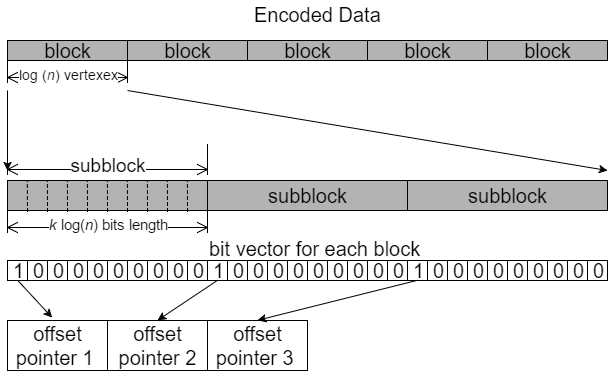
\includegraphics[width=1.0\textwidth]{indirect}
\caption{The architecture of the $indirect$ indexing structure}
\end{figure}

\bigskip

To locate the starting position of a particular vertex, we first find which block the vertex is in by dividing the vertex label by $\log(n)$ (number of vertexes in each block). Next, we check the bit vector of that block to find which subblock contains the vertex. Since we store the offset pointer for the vertexes which are the first one in their subblock, we can know the starting position of the target subblock, and then we decode the subblock. Although we will get all the adjacency lists within the subblock if do so, the degree information of each vertex is also encoded, and hence we can have the adjacency list of the target vertex easily. The bit vector of each block has $\log(n)$ bits, and each subblock is $k\log(n)$ bits long, so determining and decoding the subblock can be completed by using a lookup table, which uses constant time to decode $\Theta(\log(n))$ bits.              

\bigskip
\bigskip

\textbf{RRR-based indexing structure}. RRR is a succinct data structure which was first proposed by Raman $et \ al$.~\cite{RRR}. This data structure works on a bit sequence $S[0,...,n)$ in such a way that provides rank and select operations in $O(1)$ time at the price of $nH_{0}(S)+o(n)$ bits of cost in space, where $H_{0}(S)$ is the zero-order empirical entropy of the sequence. The RRR data structure divides the original bit sequence into several superblocks, and then divide the superblocks further into blocks. For each block, it stores a number to indicate the number of ones or zeros in the block. The number would be used as a lookup key in a table. Besides that, it also stores an offset which indicates which of the blocks the number is in. The offset is also used as an index in the table. By grouping blocks into superblock, RRR can avoid iterating over each block to conduct a rank or select query. 

\bigskip
\bigskip

RRR efficiently compresses a bit set if the set is very sparse populated, so we take advantage of this feature of RRR and implement an indexing structure based on it. The original graph is encoded into a bit sequence by using gamma codes, and we know the length of this sequence. Hence we can maintain another bit set with the same length as the encoded bit sequence, in which we set a bit to '1' if it is the starting point of an adjacency list; otherwise we set the bit to 0. By doing so, we get a bit set which is very sparse, and then we can build a RRR bit vector on this bit set. To locate a particular vertex, we only need to conduct a $select$ query on the RRR bit vector, and we will know its starting position in the encoded bit sequence in constant time. Since the encoded bit sequence has $O(n)$ bits, and for a n-bit sequence, RRR needs $nH_{0}(S)+o(n)$ bits to support constant $rank$ and $select$ queries, and we do not need to store additional information besides the RRR structure, therefore, the space cost will not exceed our bound. 

\bigskip
\bigskip

\textbf{SD Vector-based indexing structure}. SD Vector is a bit vector that can compress very sparse populated bit vectors by representing the positions of 1 by the Elias~\cite{Elias} - Fano~\cite{Fano} representation for non-decreasing sequences. Given a bit set $B[0,...n-1)$ with $m$ ones ($m << n$),   the SD Vector uses $m \log n/m  + 2m + o(m)$~\cite{Practical-Entropy} bits to store the bit set, meanwhile support constant time $rank$ and $select$ queries. The idea of SD Vector-based indexing structure is very similar to RRR-based indexing structure. We firstly maintain a bit sequence which has the same length as the encoded graph bit sequence, and next we mark the bits which indicate the starting position of an adjacency list. Then we build an SD Vector on this bit sequence. In order to locate the starting position of a particular vertex, we use the SD Vector to perform a $select$ operation which will return the expected position. 


\chapter{Experiments and Evaluation}
After implementing the data structure of Blandford $et \ al.$~\cite{compact-representation} by encoding a graph into an adjacency table as well as building an auxiliary indexing structure for supporting queries on the graph, including the alternative indexing schemes that we come up with, we would like to evaluate the performance of our implementation. In this chapter we will first describe the experimental setup which includes some our implementation details regarding succinct representations of bit vector, as well as our decoding approach. Then we will show and discuss our experiment results.

\bigskip
 
\section{Experiment Setup}

\bigskip
\textbf{RRR and SD Vectors}. As we introduced in Chapter 3, we take advantage of the features of succinct representation of bit vector to build two indexing structures: RRR-based and SD Vector-based. We used the implementation of both RRR and SD Vector structures from the succinct data structure API provided by Simon Gog~\cite{sdsl}, which presents a various of succinct representations including bit vector, integer vectors, wavelet trees, compressed suffix arrays (CSA). 

\bigskip
\bigskip

\textbf{Decoding Mechanism}. Taking advantage of the feature of Random-Access-Machine that costs constant-time to perform operations on $O(\lg n)$ bits, we can decode any $O(\lg n)$ bit words in constant time. One practical approach proposed by Blandford $et \ al$~\cite{compact-representation} is using a lookup table. In our project, the graph is Elias gamma encoded, to ensure a decoding operation on $O(\lg n)$ bits requires constant time, we implement a table to decode multiple gamma codes at once. For a fixed number of $k_{g}$, we create a table of size $2^{k_{g}}$, and use the numbers range from 0~$2^{k_{g}}$ as indexes. Each entry in the table indicates a decoding result which is represented by a 32-bit word.  

\bigskip

\begin{figure}[ht]
\centering
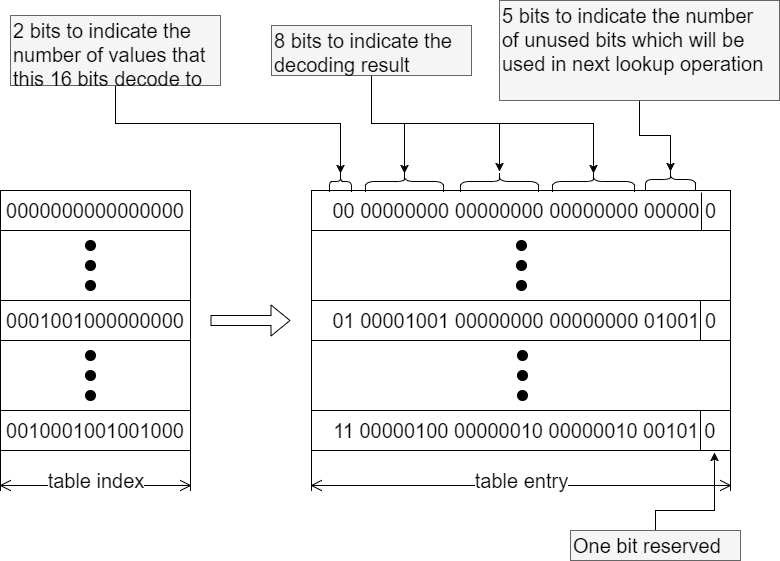
\includegraphics[width=1.0\textwidth]{Decoding}
\caption{The working mechanism of the lookup table}
\end{figure}

\bigskip

The working mechanism of this lookup table is shown in Figure 4.1 (note that we set the $k_{g}$ to 16, and limit the number of words decoded at once to 3 in our implementation): the first two bits indicate the number of values that this 16 bits decode to. If a bit block with size of 16 can not be directly decoded (e.g. the first case in the Figure 4.1, which is all zero), then the firstly two bits in the corresponding entry is set to 0, which means none of numbers can be decoded in this block. The next 24 bits ($3_{rd} - 26_{th}$ bits) indicate the three potential decoding result (if the first two bits show that only one number can be decoded, then we only look into the $3_{rd} - 11_{rd}$ bits). The next 5 bits ($27_{th} - 31_{th}$ bits) show the number of unused bits which will be used in next lookup operation, and the last bit is unused. This makes each table entry fit into 32 bits. If the first two bits indicate that no value can be directed decoded by checking this table entry, then the sequence will be decoded explicitly.

\textbf{Test Graphs}. The test graph used in our experiment come from several source: two 3D Mesh graphs from an online Graph Partitioning Archive maintained by C. Walshaw~\cite{3DMESH}, one graph from Scotch Graph Archive maintained by Dave Beckett~\cite{Scotch}, one graph from RIACS Graph Archive~\cite{RIACS}, two Gpu Layout Plugin graphs from Cytoscape online resource~\cite{Cytoscape}, and two BCS Structural Engineering Matrix graphs from Matrix Market~\cite{Matrix}. All the test graphs are undirected graphs, and a summary of general attributes of the graphs is shown in Table 4.1, giving the information about the numbers of vertexes and edges, max degrees and graph source.


\begin{table}[ht]
\centering
\caption{ Test graphs used in our experiment }
\label{graph-list}
\begin{tabular}{|l||c|c|c|c|}
\hline
\multicolumn{1}{|c||}{Graph} & Vertexes & Edges   & Max Degree & Source        \\ \hline
feocean                   & 143437   & 409593  & 6          & 3D mesh~\cite{3DMESH}        \\
m14b                      & 214765   & 1679018 & 40         & 3D mesh~\cite{3DMESH}       \\
febody                    & 45087    & 163734  & 28         & Scotch Graphs~\cite{Scotch} \\ 
wave                      & 156317   & 1059331 & 44         & RIACS Grids~\cite{RIACS}    \\
598a                      & 110971   & 741934  & 26         & Cytoscape~\cite{Cytoscape}      \\
144                       & 144649   & 1074393 & 26         & Cytoscape~\cite{Cytoscape}     \\
bcsstk30                  & 28924    & 1007284 & 218        & BCS~\cite{Matrix}    \\
bcsstk31                  & 35588    & 572914  & 188        & BCS~\cite{Matrix}     \\ \hline
\end{tabular}
\end{table}


\section{Experiment Result} 
The experiments were conducted on a Linux distribution server which contains 32 Intel Xeon E5-2650 @ 2.00GHz cores and 256 gigabytes of main memory. As we include each edge in the adjacency lists of both its endpoints, when computing the space cost measured in bits per edge, we divide the total space cost in bits by $2|E|$. Our experiment focuses on three parameters of concern: the time to construct our data structure, the time to perform queries on graphs and the space needed to encode these graphs into an adjacency table. The space cost of our data structure consists of the space for the adjacency table and the space for the indexing structure. There are a trade-off between the time to complete the construction and the space for encoding the adjacency table caused by whether to conduct the child-flipping process, as well as a trade-off between the space for the indexing data structure and the time to perform queries on graphs resulted by applying different indexing structures. Our experiments demonstrate these trade-offs.

\bigskip
\bigskip


Table 4.2 shows the time cost of constructing the compact data structure and the space needed to encoding the adjacency table. We can see that the child-flipping process causes additional time cost as a heuristic postprocessing phase, but does reduce the space cost of the adjacency table (save at most 8\% space on the febody graph, and at least 2.5\% space on the bcsstk30 graph). The space to encode the vertex degrees for each graph is listed separately, because the child-flipping process will not change the degree of each vertex, and the number of bits to encode a number is fixed (we use $2\lfloor \log d \rfloor + 1$ bits to encode a degree $d$ by using Elias gamma coding). From the table we can see that the child flipping process reduces the space cost notably without increasing the construction time greatly. Therefore, we always perform this process in subsequent studies. 

\begin{table}[]
\centering
\caption{The performance of compact mechanisms. Time is in seconds and space is in bits per edge for encoding the edges. The columns 'METIS' and 'METIS-CF' indicate that it does not perform the child flipping process and it performs the child flipping process, respectively.}
\label{compact-performance}
\begin{tabular}{|l||c|c||c|c||c|}
\cline{2-6}
\hline
\multirow{2}{*}{Graph} & \multicolumn{2}{c||}{METIS} & \multicolumn{2}{c||}{METIS-CF} & \multirow{2}{*}{Degree} \\ \cline{2-5}
                       & Time          & Space        & Time           & Space         &                         \\ \cline{6-6} \hline
feocean                & 55.69         & 8.68         & 59.51          & 8.27          & 0.86                    \\
m14b                   & 129.3         & 5.21         & 155.37         & 5.00          & 0.51                    \\
febody                 & 6.33          & 4.64         & 7.2            & 4.25          & 0.82                    \\
wave                   & 77.4          & 5.76         & 86.52          & 5.57          & 0.55                    \\
598a                   & 39.06         & 5.45         & 52.33          & 5.21          & 0.54                    \\
144                    & 67.09         & 5.32         & 84.33          & 5.13          & 0.52                    \\
bcsstk30               & 7.89          & 2.29         & 12.3           & 2.24          & 0.17                    \\
bcsstk31               & 6.61          & 2.98         & 9.02           & 2.89          & 0.30                    \\ \hline
\end{tabular}
\end{table}


\begin{table}[ht]
\centering
\caption{The space cost of different indexing structures. Space is in bits per edge.}
\label{my-label}
\begin{tabular}{|l||c||c||c||c||c|}
\hline
Graph    & Direct & Semi & Indirect & RRR & SD Vector \\ \hline
feocean  &    5.63    &   2.81   &     0.84     &  2.03   &   1.59        \\
m14b     &    2.05    &   1.02   &    0.42      &  1.01   &   0.64        \\
febody   &    4.46   &   2.23   &     0.54     &  1.33   &    1.31        \\
wave     &   2.36    &   1.18   &    0.46      &   1.14   &   0.72         \\
598a     &    2.39    &   1.19   &   0.47       &  1.10   &    0.77       \\
144      &    2.15   &   1.07   &    0.43      &  1.05    &   0.67          \\
bcsstk30 &   0.46   &   0.23   &      0.12    &   0.35   &   0.16        \\
bcsstk31 &   0.93   &   0.46   &     0.21     &  0.54   &   0.35        \\ \hline
%Avg      &    2.54   &   1.27   &     0.46     &  1.06   &    0.77       \\
%\hline
\end{tabular}
\end{table}
\bigskip

The indexing structures were built based on the ordering result after the child-flipping process. Table 4.3 illustrates the space cost of each indexing structure, while Table 4.4 illustrates the time cost to perform a bread-first search(BFS) in the graph by applying those indexing structures on the encoded adjacency table. The reason why we use BFS to measure the performance as done by Blandford $et \ al$~\cite{compact-representation} (they used DFS to measure their data structure in their experiment part) is that it requires visiting all the edges, which makes it a reasonable measure for our data structure. The BFS algorithm starts at some arbitrary vertex as the root (we use the $1_{st}$ vertex after renumbering in our project) and explores the neighbour nodes first, before moving to the neighbours at next level, with a cost of time $\Theta(|V| + |E|)$. 

\bigskip

We also compared the performance of our representation to that of an array-based adjacency list graph representation. The array-based adjacency list representation stores all the neighbours of each vertex contiguously in a large array with the neighbours placed one after the other. It also require an array to store the index of each vertex. Therefore, it use one 32-bit word to represent an edge and one 32-bit word as the index of one vertex, taking 8$|E|$ bytes (2*32*$|E|$ bits) space for the list and 4$|V|$ bytes for the indexes in total. For the BFS algorithm on any types of indexing structures, we use one bit flag to indicate whether a vertex has been visited.
\bigskip     

\begin{table}[ht]
\centering
\caption{The time performances of different indexing structures to conduct a BFS. The time cost is measured in millisecond}
\label{my-label}
\begin{tabular}{|l||c||c||c||c||c||c|}
\hline
Graph    & Array & Direct & Semi & Indirect & RRR & SD Vector \\ \hline
feocean  &   13.6    &   31.6     &   34.9   &    97.2      &  103.3   & 60.8          \\
m14b     &   36.2    &    88.5    &   93.1   &   216.8   &  251.6   &   130.7        \\
febody   &   2.5    &    7.3    &   7.9   &     27.7    &   33.7  &     13.8      \\
wave     &    19.9   &    60.8    &   66.1   &    144.8     &   176.2  &   95.1        \\
598a     &    14.5   &    42.1    &   45.9   &    102.8     &  115.0   &    65.6       \\
144      &   19.2    &    60.0    &   64.7   &     111.2     &  130.4   &  87.9         \\
bcsstk30 &   4.2    &    24.9    &   26.8   &    37.0    &   40.9  &  29.3         \\
bcsstk31 &    3.7   &    20.2    &   20.7   &     35.4    &   39.2  &  27.9         \\ \hline
%Avg      &    14.2   &    41.9    &  45.0  &          &     &           \\
%\hline
\end{tabular}
\end{table}

\bigskip

The experimental result shows that the $direct$ and $semi direct$ indexing structures give the fastest query time, but they are still slower than the array-based adjacency list representation. It is not surprising because the array-based representation has good spacial locality, which means the edges of a vertex are adjacent in memory and be loaded into cache as an array. In addition to that, the array-based representation does not need to decode the list, and hence, the array-based representation is faster than others. The $semi-direct$ indexing structure uses half of the space when compared to $direct$ indexing structure while requiring little extra time on queries. $Indirect$ indexing structure shows good space usage but it is not very efficient in queries, because it needs to decode a "subblock" rather than an adjacency list. The SD Vector-based structure outperforms the RRR-based structure in both space usage and time cost in all the test graphs, and when compared to the $Indeirect$ indexing structure, the SD Vector-based structure is more efficient in queries while requiring little more space.   

\bigskip
\begin{table}[ht]
\scriptsize
\centering
\caption{Summary of space and time performance. Space is in bits per edge and time is in millisecond. The column 'SD(DF)' means we do not encode the degree of each vertex when building the adjacency table, and then use SD Vector to build indexing structure on it.}
\label{my-label}
\begin{tabular}{|l||c|c||c|c||c|c||c|c||c|c||c|c| |c|c|}
\hline
\multirow{2}{*}{} & \multicolumn{2}{c||}{Array} & \multicolumn{2}{c||}{Direct} & \multicolumn{2}{c||}{Semi} & \multicolumn{2}{c||}{Indirect} & \multicolumn{2}{c||}{RRR} & \multicolumn{2}{c| |}{SD Vector} & \multicolumn{2}{c|}{ \textbf{ SD(DF) }} \\ \cline{2-15}
                       & \textit{T}        & \textit{S}       & \textit{T}           & \textit{S}           & \textit{T} & \textit{S}          & \textit{T}            & \textit{S}           & \textit{T}          & \textit{S}        & \textit{T} & \textit{S} & \textit{T} & \textit{S} \\ \hline
feo*          & 13.6  & 37.6   &  31.6  &  14.8  &  34.9   &   11.9  &  97.2  &  9.8  &  103.3  &  11.0  &  60.8  &  10.6  & 57.1 & 9.6            \\
m1*          & 36.2  & 34.1   &  88.5  &  7.6  &  93.1   &  6.5   &  216.8  &  5.9  &  251.6  &  6.52  &  130.7  &   6.1  & 123.2 &  5.6         \\
feb*          & 2.5   & 36.4   &  7.3   &  9.5  &  7.9   &  7.3   &  27.7  &  5.6  &  33.7  &  6.4  &  13.8  &  6.4  & 12.4 &   5.6         \\
wa*          & 19.9  & 34.3   &  60.8  &  8.5  &  66.1   &  7.3   &  144.8  &  6.5  &  176.2  &  7.2  &  95.1  &  6.8  & 89.1 &  6.3          \\
59*          & 14.5  & 34.4   &  42.1  &  8.1   &  45.9   &  6.9   &  102.8  &  6.2  &  115.0  &  6.8  &  65.6  &  6.5  & 60.9 &  5.9          \\
144           & 19.2  & 34.1   & 60.0   &  7.8  &   64.7  &  6.7   &  111.2  &  6.1  &  130.4   &  6.7  &  87.9  &  6.3   & 80.5 & 5.8          \\
b0*          & 4.2   & 32.4   &  24.9  &  2.8  &  26.8   &  2.6   &  37.0  &  2.5  &  40.9  &  2.7  &  29.3  &   2.5  & 27.1 &  2.4         \\ 
b1*          & 3.7   &  33.0  &  20.7  &  4.2  &   20.7  &   3.6  &  35.4  &  3.4  &  39.2  &  3.7  &  27.9  &   3.5  & 25.7 &  3.2         \\ \hline


\end{tabular}
\end{table}


\bigskip

Table 4.5 illustrates a summary of performance of different indexing structures associated with the encoded adjacency table built after child-flipping process. The space for each mechanism contains the space for the encoded adjacency list, the space for degree and the space for the indexing structure. We can see that the $direct$ indexing structure gives the fastest query speed while requiring the biggest space, $indirect$ indexing structure use least space while needing more time on queries, the SD Vecter-based indexing structure presents a good trade-off between the space usage and query efficiency. 

\bigskip
\bigskip

To ensure the degree queries can be completed in constant time, we encode the degree of each vertex at the beginning of each corresponding adjacency list, but for the adjacency queries and neighbouring list queries, the degree information is not necessary. In the last two columns (under the 'SD(DF)' column, 'SD(DF)' means 'SD Vector(degree-free)') of the Table 4.5, we present the time and the space of conducting the BFS algorithm and building the adjacency tables, respectively. We can see that the space and time are further saved when the degree information is not encoded, this is because the neighbouring list queries needed by the BFS algorithm (require decoding the adjacency list for each vertex) is more efficient without a degree encoded at the beginning of each adjacency list. But note that although the absence of the degree information may reduce the space to encode the adjacency table and the time for adjacency and neighbouring list queries, it can not make the degree queries be completed in constant time, because it needs to decode the entire adjacency list first, then it can know the number of neighbours in that list. The reason why we only chose to use SD Vector-based indexing structure to demonstrate the trade-off of the space to encode the adjacency and the time to conduct different queries on graphs caused by whether encoding the degree information into the adjacency table is because: 1) our experiment demonstrates that the SD Vector-based indexing structure outperforms the RRR-based indexing structure greatly; 2) the $direct$ and $semi-direct$ indexing structures exceed our space bound; 3) the degree information for each vertex is necessary for $indirect$ indexing structure.  


\chapter{Conclusions and Future Work}

In this project, we focused on how to represent a separable graph compactly while supporting efficient queries. Our theoretical basis came from a previous work conducted by Blandford $et \ al.$~\cite{compact-representation}, which provided the theory of using vertex separators to compactly represent the graph. The representation takes $O(n)$ bits, meanwhile using constant time to support degree or adjacency queries, and neighbour listing for one vertex in constant time per neighbour. 

\bigskip
\bigskip

We first conducted a survey on the research related to succinct data structure on planar graphs, as well as some succinct representations on bit vector like RRR. Then we focused on the representation of separable graph. 

\bigskip
\bigskip

Next, we used the METIS$\_$API to partition the graph by removing some amount of edges recursively, and construct the edge separator tree for the graph. To reduce the space of difference encoding, we conducted a heuristic postprocessing phase called "child-flipping" on the edge separator tree. We used Elias gamma codes to encode the adjacency list of each vertex, and concatenated all the adjacency lists to an adjacency table.

\bigskip
\bigskip

Then we implemented several indexing structures to support adjacency queries, degree queries and neighbourhood queries in constant time. Besides the three indexing structure mentioned in the work of Blanddford $et \ al.$, we implemented other two structures based on succinct representations on bit vectors.

\bigskip
\bigskip

Finally we conducted some experiments to measure the performance of our representation. The experiments demonstrated the trade-off between the space cost to encode the adjacency table and the time to construct the data structure, as well as the trade-off between the space cost and time of queries by different indexing structures. Compared to the array-based adjacency list representation, our implementation reduces space usage by almost an order of magnitude, while supporting bread-first search in acceptable running time.

\bigskip
\bigskip

For the future work, we intend to implement the separator tree by using the vertex separators, and apply different coding schemes like delta~\cite{Elias}, Huffman coding, etc. Besides that, we can try to design and implement more indexing structures to investigate more about the time/space trade-offs.
 
\bibliographystyle{plain}
\bibliography{bib}

\end{document}
